\documentclass{beamer}
\usetheme{Boadilla}
\usepackage[norsk]{babel}
\usepackage{natbib}
\usepackage[utf8]{inputenc}
\usepackage{url}
\usepackage{hyperref}
\hypersetup{colorlinks=false, citebordercolor={1 1 1}}
\title[Haptikk og digitale musikkinstrumenter]{Haptikk og digitale musikkinstrumenter}
\author[Håkon Knutzen]{Håkon Knutzen}
\institute[UiO]{
	\includegraphics[scale=.15]{figs/uiologo-45mm.pdf}
}
\date{26. september, 2014}

\begin{document}

\begin{frame}
	\titlepage
\end{frame}

\begin{frame}
	\frametitle{Begreper}
	\begin{itemize}[<+->]
		\item Feedback (tilbakemelding)
		\item Haptikk, \emph{haptein} (gresk: å ta): ``Haptisk, i kunstvitenskapelig sammenheng det som kan fattes med følesansen. Skulptur er en haptisk kunstart, \emph{musikk ikke}.''\footnote{\url{https://snl.no/haptisk [min kursivering]}}
		\item Taktil, \emph{tactilis} (latin: å ta)
		\item Haptisk feedback ofte brukt som en samlebetegnelse for \emph{kinestetisk} og \emph{taktil} feedback \citep{oakley_putting_2000}
	\end{itemize}
\end{frame}

\begin{frame}
	\frametitle{Kinestetisk og taktil sansning}
	\begin{itemize}[<+->]
		\item Kinestetisk sansning: Kraft mot muskler og ledd
		\item Taktil sansning: Sansning av stimuli med med huden: tekstur, vibrasjoner, temperatur og smerte
		\item Rask sansemodalitet
		\item Mekanoreseptorer, forskjellige typer som responderer på ulike frekvenser
		\item \emph{Vibro}taktil
	\end{itemize}
\end{frame}

\begin{frame}
	\frametitle{Taktil sansning I}
		\begin{itemize}[<+->]
		\item Fingrene er mest sensitive for taktil musikalsk feedback (17000 mekanoreseptorer i hånda)
		\item Kan sanse vibrasjoner mellom 0--1000 Hz (varierer i litteraturen)
		\item Vibrasjoner fra instrumenter opptrer over terskelen for stimuli som kan sanses \citep{askenfelt_vibration_1992}
	\end{itemize}
\end{frame}

\begin{frame}
	\frametitle{Taktil sansning II}
	\begin{figure}
		\includegraphics[scale=.3]{figs/verrillo.png}
		\caption{\citep[p.\ 287]{verrillo_vibration_1992}}
	\end{figure}		
\end{frame}



\begin{frame}
	\frametitle{Kvalitative observasjoner}
	\begin{itemize}[<+->]
		\item Instrumentell betydning:
		\begin{itemize}
			\item Strykeorkestre \citep{askenfelt_vibration_1992}
			\item Navigering på halsen på en gitar \citep{kvifte_instruments_2007}
			\item Barregrep, skurring
		\end{itemize}
		\item Følelsen av å spille på et instrument \citep{chafe_musical_1996}
	\end{itemize}
\end{frame}

\begin{frame}
	\frametitle{Kvantitative observasjoner}
	\begin{figure}
		\includegraphics[scale=.25]{figs/chafe.png}
		\vspace{-15pt}
		\caption{\citep[p.\ 76]{chafe_tactile_1993}}
	\end{figure}
\end{frame}

%------brudd i taktil kobling, problemområde for digitale instrumenter
\begin{frame}
	\frametitle{Feedback}
	\begin{figure}
		\includegraphics[scale=.23]{figs/broken.png}
		\caption{\citep[p.\ 356]{rovan_typology_2000}}
	\end{figure}
\end{frame}

\begin{frame}[allowframebreaks]
	\frametitle{Eksempler}
	\begin{figure}
		\includegraphics[scale=.31]{figs/ERGOS_Photo02.jpg}
		\caption{ERGOS\footnote{\url{http://acroe.imag.fr/ergos-technologies/index.php?idp=1}}}
	\end{figure}
	
	\begin{figure}
		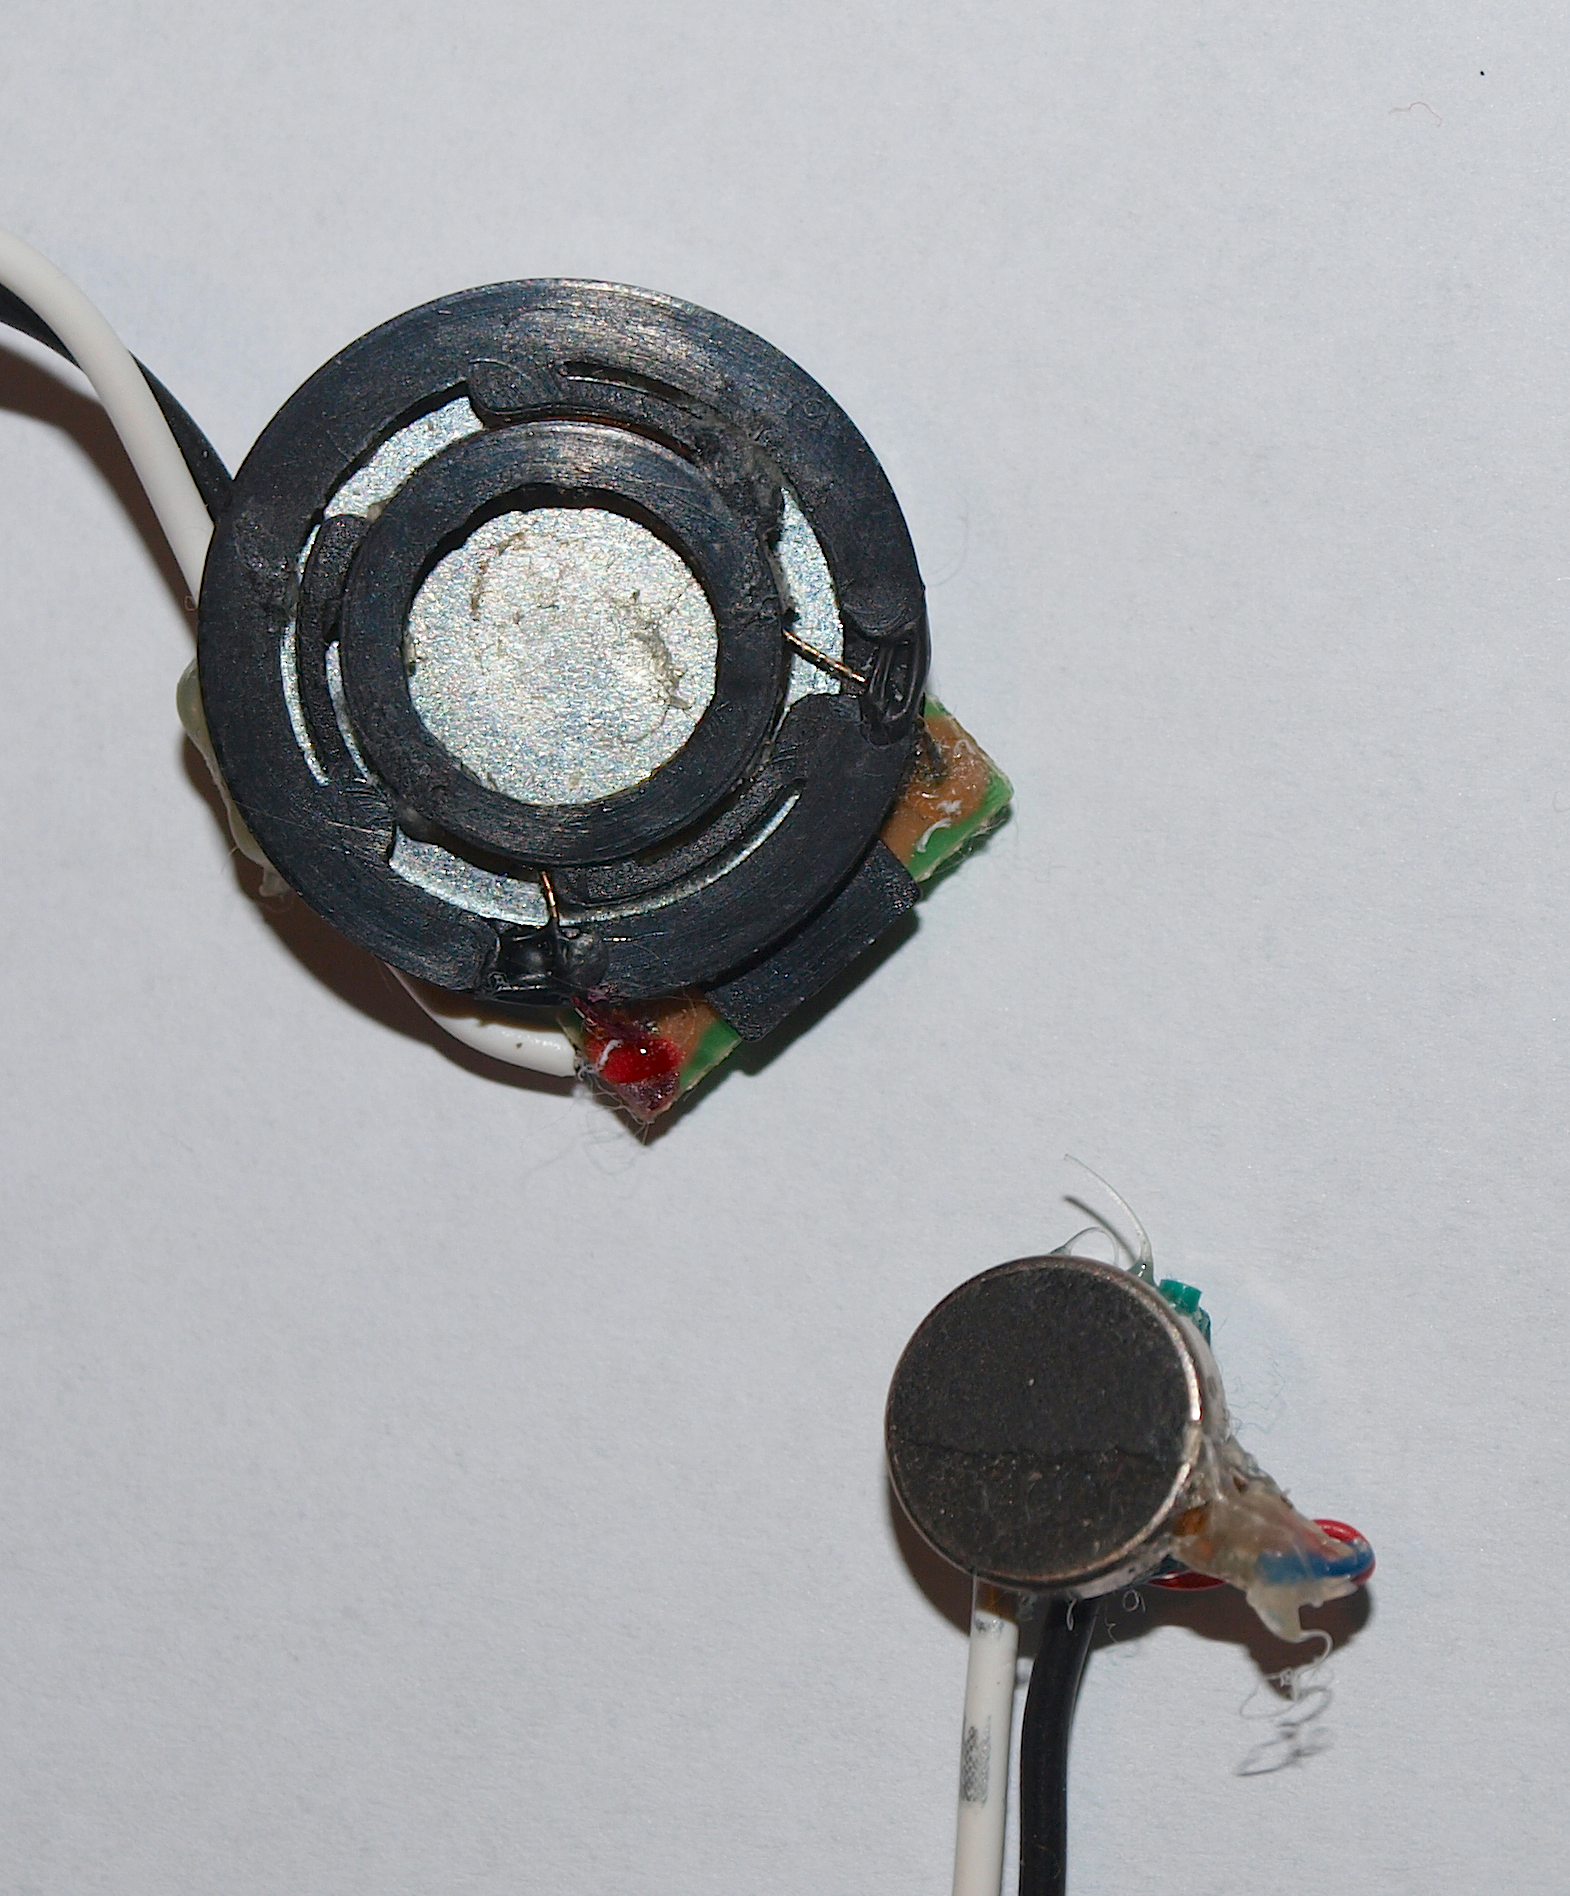
\includegraphics[scale=.11]{figs/actuators.png}
	\end{figure}
	\begin{figure}
		\includegraphics[scale=.39]{figs/ccloseups.png}
		\caption{\citep{knutzen2013,knutzen_vibrotactile_2014}}
	\end{figure}
	\begin{figure}
		\includegraphics[scale=.2]{figs/giordanoact.png}
		\caption{\citep{schumacher_vibrotactile_2013}}
	\end{figure}
\end{frame}

\begin{frame}
	\frametitle{Mapping}
	\begin{figure}
		\includegraphics[scale=.25]{figs/webmapper.png}
		\caption{Libmapper\footnote{\url{http://libmapper.github.io/}}}
	\end{figure}
\end{frame}

\begin{frame}
	\frametitle{Oppsummering}
	\begin{itemize}
		\item Haptisk sansning forekommer i musikalsk praksis
		\item Observasjon viser at man kan sanse taktile stimuli som oppfører seg i tråd med hvordan parametre i musikken oppfører seg
		\item Mange drar nytte av haptisk feedback
		\item Lite utnyttet i digitale musikkinstrumenter
		\item Ganske ungt forskningsfelt
	\end{itemize}
\end{frame}

\begin{frame}[allowframebreaks]
	\frametitle{Referanser}
	\bibliographystyle{apalike}
	\bibliography{zotero,utenom}
\end{frame}

\end{document}